% To je predloga za poročila o domačih nalogah pri predmetih, katerih
% nosilec je Blaž Zupan. Seveda lahko tudi dodaš kakšen nov, zanimiv
% in uporaben element, ki ga v tej predlogi (še) ni. Več o LaTeX-u izveš na
% spletu, na primer na http://tobi.oetiker.ch/lshort/lshort.pdf.
%
% To predlogo lahko spremeniš v PDF dokument s pomočjo programa
% pdflatex, ki je del standardne instalacije LaTeX programov.

\documentclass[a4paper,11pt]{article}
\usepackage{a4wide}
\usepackage{fullpage}
\usepackage[utf8x]{inputenc}
\usepackage[slovene]{babel}
\selectlanguage{slovene}
\usepackage[toc,page]{appendix}
\usepackage[pdftex]{graphicx} % za slike
\usepackage{setspace}
\usepackage{color}
\definecolor{light-gray}{gray}{0.95}
\usepackage{listings} % za vključevanje kode
\usepackage{hyperref}
\renewcommand{\baselinestretch}{1.2} % za boljšo berljivost večji razmak
\renewcommand{\appendixpagename}{Priloge}

\lstset{ % nastavitve za izpis kode, sem lahko tudi kaj dodaš/spremeniš
language=Python,
basicstyle=\footnotesize,
basicstyle=\ttfamily\footnotesize\setstretch{1},
backgroundcolor=\color{light-gray},
}

\title{Informativnost značilk pri napovedovanju posameznih tem}
\author{Gregor Majcen (63070199)}
\date{\today}

\begin{document}

\maketitle

\section{Izjava o izdelavi domače naloge}
Domačo nalogo in pripadajoče programe sem izdelal sam.

\section{Uvod}
Druga domača naloga je namenjena raziskovanju diskretnih značilk (atributov). Raziskovali bomo informativnost (krat. I) in koliko nam to sploh pomeni. Vzemimo na primer I=0.1 in tu se pojavi najtežje vprašanje: je to vredu ali ne? Ker je vse skupaj odvisno od primera na žalost ne moremo odgovoriti, lahko pa testiramo s permutacijskim testom.

\section{Metode}
\begin{description}
\item[Mera nedoločenosti ali Entropija: ]$H(A) = -\sum_{i=1}^n(p(x_i) * \log_2(x_i))$
\item[Informacijski prispekvek: ] $I(C;A) = H(C) - H(C|A)$
\end{description}
\ \\
Vzemimo na primer razred c40 in atribut D\_0. $C = c40$ in $A = D\_0$. 
\ \\
\begin{tabular}{|r|l|}
  \hline
  1498 & $C=F$ \\
  502 & $C=T$ \\
  \hline
\end{tabular}
$H(C) = H({1498\over2000}, {502\over2000}) = -({1498\over2000}*\log_2{1498\over2000} + {502\over2000}*\log_2{502\over2000}) = 0.8128592431848387$
\ \\
\begin{tabular}{|r|l|}
  \hline
  9 & $A>0$ in $C=F$ \\
  1 & $A>0$ in $C=T$ \\
  1489 & $A=0$ in $C=F$ \\
  501 & $A=0$ in $C=T$ \\
  \hline
\end{tabular}
\ \\
$H(C|A) = {10\over2000}*H({9\over2000}, {1\over2000}) + {1990\over2000}*H({1489\over2000}, {501\over2000}) =$
$ -{10\over2000}({9\over2000}*\log_2{9\over2000} + {1\over2000}*\log_2{1\over2000}) - {1990\over2000}({1489\over2000}*\log_2{1489\over2000} + {501\over2000}*\log_2{501\over2000}) = 0.8132959330794926$
\ \\
$I(A) = H(C|A) - H(C) = 0.8132959330794926 - 0.8128592431848387 = 0.0004366898946538411$
Orange.feature.scoring.InfoGain(a, data) $ = 0.0005311369895935059$

\begin{description}
\item[Permutacijski test] P-test nam odgovori na vprašanje, ali je naš I dober ali slab in sicer s pomočjo naključnih primerov. Ideja je v tem, da izračunamo čimveč informacijskih prispevkov naključnih primerov (v našem primeru 100 in 500) ter primerjamo z našim originalnim rezultatom. Želimo, da so naključni primeri zmerom slabši. S tem bi pokazali, da je naš atribut zares dober. Ker na žalost vedno ni tako, lahko določimo mejo, imenovana alfa. Alfa (v našem primeru 0.05 in 0) nam pove, koliko procentov naključnih boljših še toleriramo.
\item[Programiranje: ] Za InfoGain je uporabljena funkcija iz Orange (kar se je na koncu izkazala, da je malo počasna, ampak takrat sem že pridobil vse potrebne podatke). Ker je 500 permutacij veliko in dolgotrajno, se je vse skupaj poganjalo v večih kosih in s tem na več jedrih, kar je zelo pohitrilo izvajanje. Kot optimizacijo sem uporabljal numpy in celotno kodo poskusil stisniti v čimmanj vrstic (in še manj for zank, ki so v pythonu zelo počasne). Za vsak razred sem po končanem izvajanju shranil rezultate na disk kot npy (numpy format) in si s tem zagotovil podatke brez ponovnega dolgotrajnega računanja.
\end{description}

\section{Rezultati}
\begin{figure}[h!]
\begin{center}
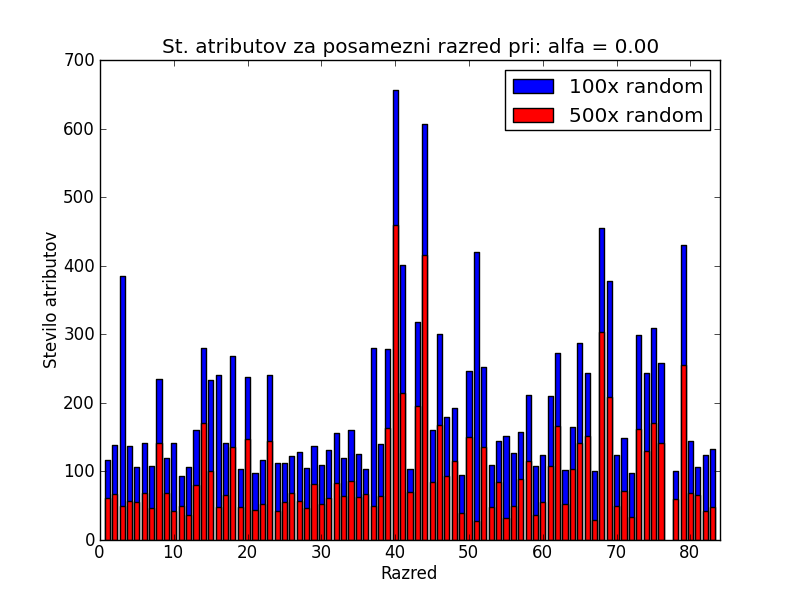
\includegraphics[scale=0.4]{1.png}
\end{center}
Tukaj imamo alfo enako nič, kar pomeni da ne toleriramo nobenega boljšega naključnega. Iz grafa je zelo lepo razvidno, da če postavimo alfo na nič še ne pomeni da je rezultat 100\%. Za tak rezultat bi morali narediti vse možne kombinacije (kar jih je veliko več kot 100 in 500).
\begin{center}
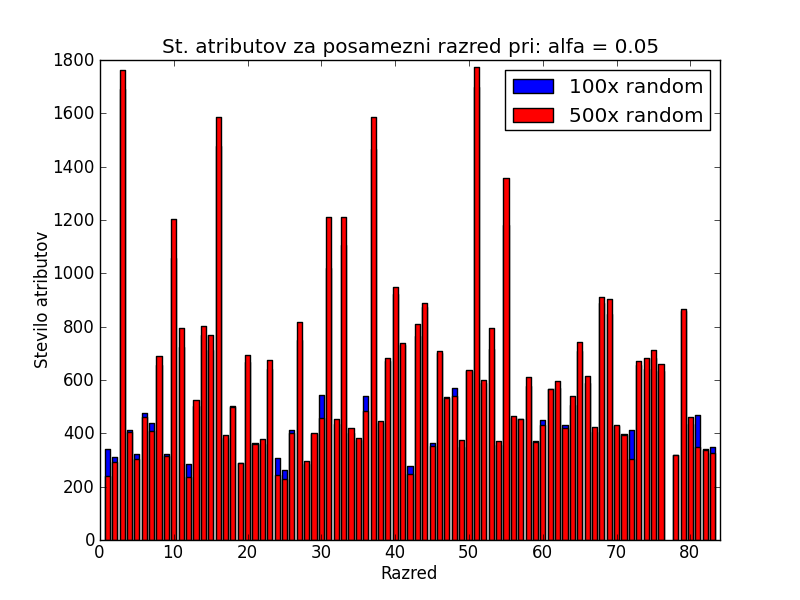
\includegraphics[scale=0.3]{2.png}
\end{center}
Na videz čisto drugačen graf, kot je prikazan zgoraj, ampak je edina razlika s 5\% puščanjem naključnih boljših. Lepo je razvidno, da z zviševanjem številu naključnih ne pridobimo več tako zelo veliko kot izgubimo na času, tako da se lahko zamislimo, kaj nam je bolj pomembno.
\end{figure}

\begin{figure}
\begin{center}
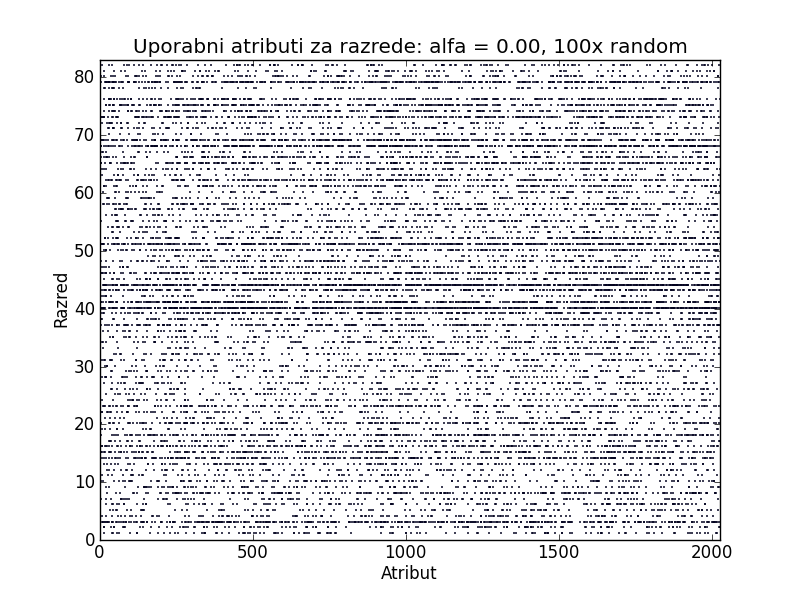
\includegraphics[scale=0.5]{3.png}
\caption{Tabela dobrih atributov pri 100x p-testu in alfa=0}
\end{center}
Bolj kot so pogoste pikice vertikalno, boljši je naš atribut. Lahko pa tudi razmišljamo obratno. Bolj pogoste horizontalne pikice nam povedo, s koliko dobrimi atributi je naš razred zastavljen. Primerjava z 500x p-testom je vidna na Sliki 3.
\begin{center}
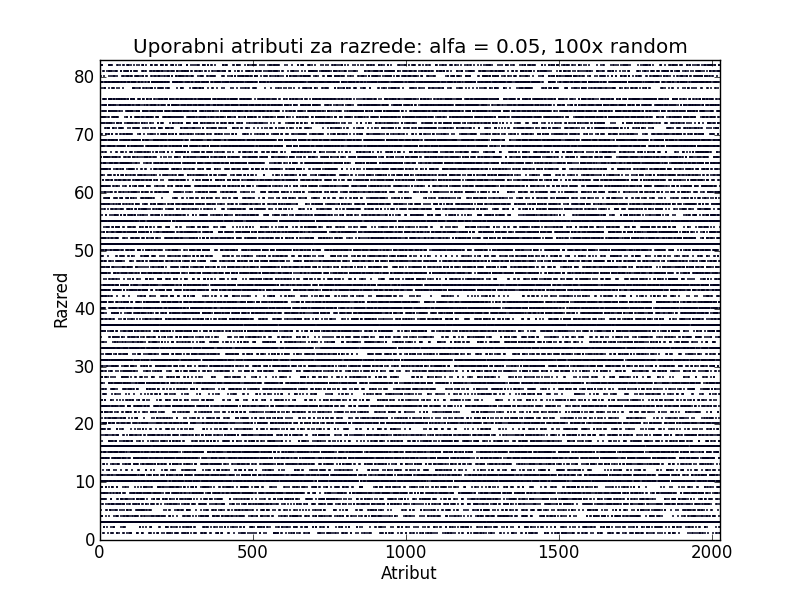
\includegraphics[scale=0.5]{4.png}
\caption{Tabela dobrih atributov pri 100x p-testu in alfa=0.05}
\end{center}
Če pa alfo povečamo za 5\% pa ne vidimo več tako lepe slike. So pa zelo lepo razvidni zelo slabi atributi ali pa razredi z zelo malo uporabnimi atributi. Primerjava z 500x p-testom je vidna na Sliki 4.
\end{figure}

\begin{figure}
\begin{center}
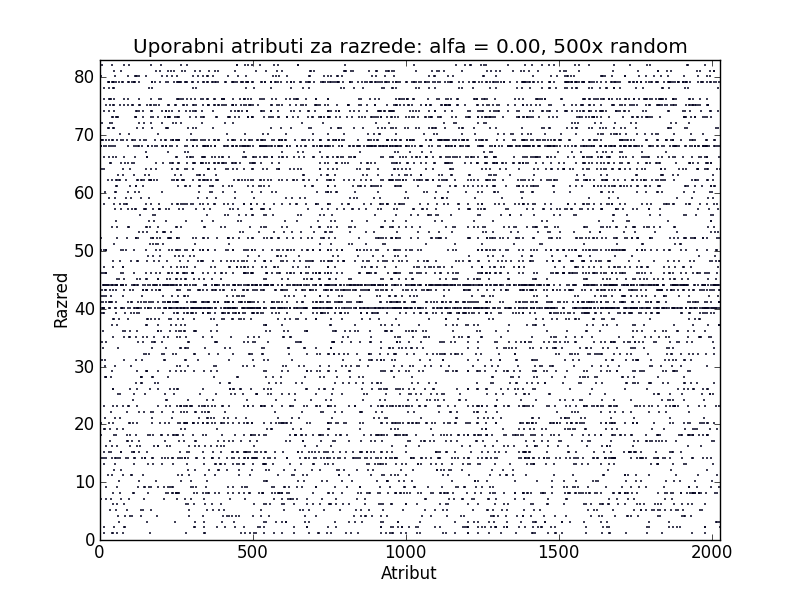
\includegraphics[scale=0.5]{5.png}
\caption{Tabela dobrih atributov pri 500x p-testu in alfa=0}
\end{center}
Kot je že napisano pri Sliki 1, so tu rezultati večjega p-testa. Vse skupaj je zelo podobno, ampak je vseeno razvidno, da smo našli kar nekaj atributov, ki so naključno boljši. 
\begin{center}
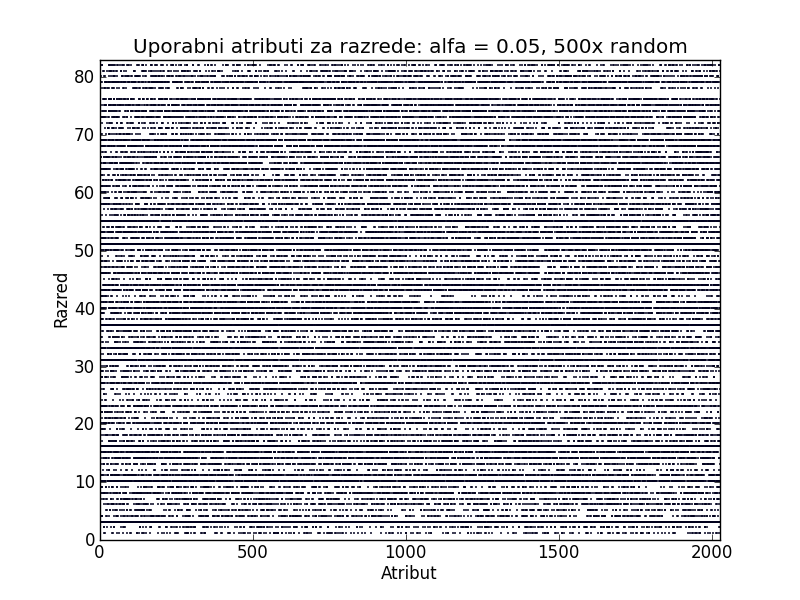
\includegraphics[scale=0.5]{6.png}
\caption{Tabela dobrih atributov pri 500x p-testu in alfa=0.05}
\end{center}
Če primerjamo s Sliko 2, vidimo da sta si zelo podobni. Iz tega je potegnjen zaključek, da većji kot je alfa, manjši p-test potrebujemo za dokaj podobne rezultate in seveda brez dodatno izgubljenega časa.
\end{figure}

\end{document}
